\chapter{CvAux}

\section{Stereo Correspondence Functions}

\cvfunc{FindStereoCorrespondence} 

Calculates disparity for stereo-pair

\cvexp{
cvFindStereoCorrespondence(
                   \par const  CvArr* leftImage, \par const  CvArr* rightImage,
                   \par int     mode, \par CvArr*  depthImage,
                   \par int     maxDisparity,
                   \par double  param1, \par double  param2, \par double  param3,
                   \par double  param4, \par double  param5  );

}{CPP}{PYTHON}

\begin{description}
\cvarg{leftImage}{Left image of stereo pair, rectified grayscale 8-bit imagerightImage}
\cvarg{rightImage}{Right image of stereo pair, rectified grayscale 8-bit imagemode}
\cvarg{mode}{Algorithm used to find a disparity (now only CV\_DISPARITY\_BIRCHFIELD is supported)}
\cvarg{depthImage}{Destination depth image, grayscale 8-bit image that codes the scaled disparity, so that the zero disparity (corresponding to the points that are very far from the cameras) maps to 0, maximum disparity maps to 255.}
\cvarg{maxDisparity}{Maximum possible disparity. The closer the objects to the cameras, the larger value should be specified here. Too big values slow down the process significantly.}
\cvarg{param1, param2, param3, param4, param5}{- parameters of algorithm. For example, param1 is the constant occlusion penalty, param2 is the constant match reward, param3 defines a highly reliable region (set of contiguous pixels whose reliability is at least param3), param4 defines a moderately reliable region, param5 defines a slightly reliable region. If some parameter is omitted default value is used. In Birchfield's algorithm param1 = 25, param2 = 5, param3 = 12, param4 = 15, param5 = 25 (These values have been taken from "Depth Discontinuities by Pixel-to-Pixel Stereo" Stanford University Technical Report STAN-CS-TR-96-1573, July 1996.)}
\end{description}

The function \texttt{cvFindStereoCorrespondence} calculates disparity map for two rectified grayscale images.

Example. Calculating disparity for pair of 8-bit color images

\begin{lstlisting}
/*---------------------------------------------------------------------------------*/
IplImage* srcLeft = cvLoadImage("left.jpg",1);
IplImage* srcRight = cvLoadImage("right.jpg",1);
IplImage* leftImage = cvCreateImage(cvGetSize(srcLeft), IPL\_DEPTH\_8U, 1);
IplImage* rightImage = cvCreateImage(cvGetSize(srcRight), IPL\_DEPTH\_8U, 1);
IplImage* depthImage = cvCreateImage(cvGetSize(srcRight), IPL\_DEPTH\_8U, 1);

cvCvtColor(srcLeft, leftImage, CV\_BGR2GRAY);
cvCvtColor(srcRight, rightImage, CV\_BGR2GRAY);

cvFindStereoCorrespondence( leftImage, rightImage, CV\_DISPARITY\_BIRCHFIELD, depthImage, 50, 15, 3, 6, 8, 15 );
/*---------------------------------------------------------------------------------*/

\end{lstlisting}

And here is the example stereo pair that can be used to test the example
\newline
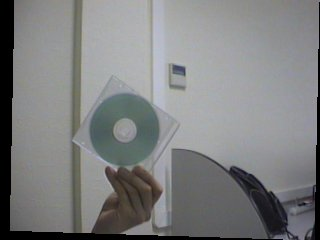
\includegraphics{pics/left.jpg}
\newline
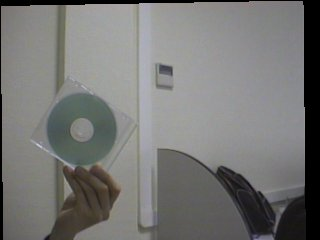
\includegraphics{pics/right.jpg}


\section{View Morphing Functions}

\cvfunc{MakeScanlines}

Calculates scanlines coordinates for two cameras by fundamental matrix

\cvexp{
void cvMakeScanlines( \par const CvMatrix3* matrix, \par CvSize img\_size, \par int* scanlines1,
                      \par int* scanlines2, \par int* lengths1, \par int* lengths2, \par int* line\_count );

}{CPP}{PYTHON}

\begin{description}
\cvarg{matrix}{Fundamental matrix.}
\cvarg{imgSize}{Size of the image.}
\cvarg{scanlines1}{Pointer to the array of calculated scanlines of the first image.}
\cvarg{scanlines2}{Pointer to the array of calculated scanlines of the second image.}
\cvarg{lengths1}{Pointer to the array of calculated lengths (in pixels) of the first image scanlines.}
\cvarg{lengths2}{Pointer to the array of calculated lengths (in pixels) of the second image scanlines.}
\cvarg{line\_count}{Pointer to the variable that stores the number of scanlines.}
\end{description}

The function \texttt{cvMakeScanlines} finds coordinates of scanlines for two images.

This function returns the number of scanlines. The function does nothing except calculating the number of scanlines if the pointers \texttt{scanlines1} or \texttt{scanlines2} are equal to zero.

\cvfunc{PreWarpImage}

Rectifies image

\cvexp{
void cvPreWarpImage( \par int line\_count, \par IplImage* img, \par uchar* dst,
                     \par int* dst\_nums, \par int* scanlines );

}{CPP}{PYTHON}

\begin{description}
\cvarg{line\_count}{Number of scanlines for the image.}
\cvarg{img}{Image to prewarp.}
\cvarg{dst}{Data to store for the prewarp image.}
\cvarg{dst\_nums}{Pointer to the array of lengths of scanlines.}
\cvarg{scanlines}{Pointer to the array of coordinates of scanlines.}
\end{description}

The function \texttt{cvPreWarpImage} rectifies the image so that the scanlines in the rectified image are horizontal. The output buffer of size \texttt{max(width,height)*line\_count*3} must be allocated before calling the function.

\cvfunc{FindRuns}

Retrieves scanlines from rectified image and breaks them down into runs

\cvexp{
void cvFindRuns( \par int line\_count, \par uchar* prewarp1, \par uchar* prewarp2,
                 \par int* line\_lengths1, \par int* line\_lengths2,
                 \par int* runs1, \par int* runs2,
                 \par int* num\_runs1, \par int* num\_runs2 );

}{CPP}{PYTHON}

\begin{description}
\cvarg{line\_count}{Number of the scanlines.}
\cvarg{prewarp1}{Prewarp data of the first image.}
\cvarg{prewarp2}{Prewarp data of the second image}.
\cvarg{line\_lengths1}{Array of lengths of scanlines in the first image.}
\cvarg{line\_lengths2}{Array of lengths of scanlines in the second image.}
\cvarg{runs1}{Array of runs in each scanline in the first image.}
\cvarg{runs2}{Array of runs in each scanline in the second image.}
\cvarg{num\_runs1}{Array of numbers of runs in each scanline in the first image.}
\cvarg{num\_runs2}{Array of numbers of runs in each scanline in the second image.}
\end{description}

The function \texttt{cvFindRuns} retrieves scanlines from the rectified image and breaks each scanline down into several runs, that is, series of pixels of almost the same brightness.

\cvfunc{DynamicCorrespondMulti}

Finds correspondence between two sets of runs of two warped images

\cvexp{
void cvDynamicCorrespondMulti( \par int line\_count, \par int* first, \par int* first\_runs,
                               \par int* second, \par int* second\_runs,
                               \par int* first\_corr, \par int* second\_corr );

}{CPP}{PYTHON}

\begin{description}
\cvarg{line\_count}{Number of scanlines.}
\cvarg{first}{Array of runs of the first image.}
\cvarg{first\_runs}{Array of numbers of runs in each scanline of the first image.}
\cvarg{second}{Array of runs of the second image.}
\cvarg{second\_runs}{Array of numbers of runs in each scanline of the second image.}
\cvarg{first\_corr}{Pointer to the array of correspondence information found for the first runs.}
\cvarg{second\_corr}{Pointer to the array of correspondence information found for the second runs.}
\end{description}

The function \texttt{cvDynamicCorrespondMulti} finds correspondence between two sets of runs of two images. Memory must be allocated before calling this function. Memory size for one array of correspondence information is

\texttt{max( width,height )* numscanlines*3*sizeof ( int ).} 


\cvfunc{MakeAlphaScanlines}

Calculates coordinates of scanlines of image from virtual camera

\cvexp{
void cvMakeAlphaScanlines( \par int* scanlines1, \par int* scanlines2,
                           \par int* scanlinesA, \par int* lengths,
                           \par int line\_count, \par float alpha );

}{CPP}{PYTHON}

\begin{description}
\cvarg{scanlines1}{Pointer to the array of the first scanlines.}
\cvarg{scanlines2}{Pointer to the array of the second scanlines.}
\cvarg{scanlinesA}{Pointer to the array of the scanlines found in the virtual image.}
\cvarg{lengths}{Pointer to the array of lengths of the scanlines found in the virtual image.}
\cvarg{line\_count}{Number of scanlines.}
\cvarg{alpha}{Position of virtual camera \texttt{($0.0 - 1.0$)}.} 
\end{description}

The function \texttt{cvMakeAlphaScanlines} finds coordinates of scanlines for the virtual camera with the given camera position.

Memory must be allocated before calling this function. Memory size for the array of correspondence runs is \texttt{numscanlines*2*4*sizeof(int)}. Memory size for the array of the scanline lengths is \texttt{numscanlines*2*4*sizeof(int).}

\cvfunc{MorphEpilinesMulti}

Morphs two pre-warped images using information about stereo correspondence

\cvexp{
void cvMorphEpilinesMulti( \par int line\_count, \par uchar* first\_pix, \par int* first\_num,
                           \par uchar* second\_pix, \par int* second\_num,
                           \par uchar* dst\_pix, \par int* dst\_num,
                           \par float alpha, \par int* first, \par int* first\_runs,
                           \par int* second, \par int* second\_runs,
                           \par int* first\_corr, \par int* second\_corr );

}{CPP}{PYTHON}

\begin{description}
\cvarg{line\_count}{Number of scanlines in the prewarp image.}
\cvarg{first\_pix}{Pointer to the first prewarp image.}
\cvarg{first\_num}{Pointer to the array of numbers of points in each scanline in the first image.}
\cvarg{second\_pix}{Pointer to the second prewarp image.}
\cvarg{second\_num}{Pointer to the array of numbers of points in each scanline in the second image.}
\cvarg{dst\_pix}{Pointer to the resulting morphed warped image.}
\cvarg{dst\_num}{Pointer to the array of numbers of points in each line.}
\cvarg{alpha}{Virtual camera position \texttt{($0.0 - 1.0$)}.}
\cvarg{first}{First sequence of runs.}
\cvarg{first\_runs}{Pointer to the number of runs in each scanline in the first image.}
\cvarg{second}{Second sequence of runs.}
\cvarg{second\_runs}{Pointer to the number of runs in each scanline in the second image.}
\cvarg{first\_corr}{Pointer to the array of correspondence information found for the first runs.}
\cvarg{second\_corr}{Pointer to the array of correspondence information found for the second runs.}
\end{description}

The function \texttt{cvMorphEpilinesMulti} morphs two pre-warped images using information about correspondence between the scanlines of two images.

\cvfunc{PostWarpImage}

Warps rectified morphed image back

\cvexp{
void cvPostWarpImage( \par int line\_count, \par uchar* src, \par int* src\_nums,
                      \par IplImage* img, \par int* scanlines );

}{CPP}{PYTHON}

\begin{description}
\cvarg{line\_count}{Number of the scanlines.}
\cvarg{src}{Pointer to the prewarp image virtual image.}
\cvarg{src\_nums}{Number of the scanlines in the image.}
\cvarg{img}{Resulting unwarp image.}
\cvarg{scanlines}{Pointer to the array of scanlines data.}
\end{description}

The function \texttt{cvPostWarpImage} warps the resultant image from the virtual camera by storing its rows across the scanlines whose coordinates are calculated by \cross{MakeAlphaScanlines}.

\cvfunc{DeleteMoire}

Deletes moire in given image

\cvexp{
void cvDeleteMoire( IplImage* img );

}{CPP}{PYTHON}

\begin{description}
\cvarg{img}{Image.}
\end{description}

The function \texttt{cvDeleteMoire} deletes moire from the given image. The post-warped image may have black (un-covered) points because of possible holes between neighboring scanlines. The function deletes moire (black pixels) from the image by substituting neighboring pixels for black pixels. If all the scanlines are horizontal, the function may be omitted.

\section{3D Tracking Functions} % XXX Weird URL Formatting, /../?

The section discusses functions for tracking objects in 3d space using a stereo camera. Besides C API, there is DirectShow
\url{http://opencvlibrary.sourceforge.net/../appPage/3dTracker/3dTrackerFilter.htm}
filter and the wrapper application
\url{http://opencvlibrary.sourceforge.net/../appPage/3dTracker/3dTracker.htm}.
\url{http://opencvlibrary.sourceforge.net/../appPage/3dTracker/3dTrackerTesting.htm} you may find a description how to test the filter on sample data.

\cvfunc{3dTrackerCalibrateCameras} % XXX URL Formatting

Simultaneously determines position and orientation of multiple cameras

\cvexp{
CvBool cv3dTrackerCalibrateCameras(\par int num\_cameras,
           \par const Cv3dTrackerCameraIntrinsics camera\_intrinsics[],
           \par CvSize checkerboard\_size,
           \par IplImage *samples[],
           \par Cv3dTrackerCameraInfo camera\_info[]);

}{CPP}{PYTHON}

\begin{description}
\cvarg{num\_cameras}{the number of cameras to calibrate. This is the size of each of the three array parameters.}
\cvarg{camera\_intrinsics}{camera intrinsics for each camera, such as determined by CalibFilter.}
\cvarg{checkerboard\_size}{the width and height (in number of squares) of the checkerboard.}
\cvarg{samples}{images from each camera, with a view of the checkerboard.}
\cvarg{camera\_info}{filled in with the results of the camera calibration. This is passed into \cross{3dTrackerLocateObjects} to do tracking.}
\end{description}

The function \texttt{cv3dTrackerCalibrateCameras} searches for a checkerboard of the specified size in each of the images. For each image in which it finds the checkerboard, it fills in the corresponding slot in \texttt{camera\_info} with the position and orientation of the camera relative to the checkerboard and sets the \texttt{valid} flag. If it finds the checkerboard in all the images, it returns true; otherwise it returns false.

This function does not change the members of the \texttt{camera\_info} array that correspond to images in which the checkerboard was not found. This allows you to calibrate each camera independently, instead of simultaneously. To accomplish this, do the following:
\begin{enumerate}
\item Clear all the \texttt{valid} flags before calling this function the first time;
\item Call this function with each set of images;
\item Check all the \texttt{valid} flags after each call. When all the \texttt{valid} flags are set, calibration is complete.
\end{enumerate}

Note that this method works well only if the checkerboard is rigidly mounted; if it is handheld, all the cameras should be calibrated simultanously to get an accurate result. To ensure that all cameras are calibrated simultaneously, ignore the \texttt{valid} flags and use the return value to decide when calibration is complete.

\cvfunc{3dTrackerLocateObjects}

Determines 3d location of tracked objects

\cvexp{
int  cv3dTrackerLocateObjects(\par int num\_cameras,
         \par int num\_objects,
         \par const Cv3dTrackerCameraInfo camera\_info[],
         \par const Cv3dTracker2dTrackedObject tracking\_info[],
         \par Cv3dTrackerTrackedObject tracked\_objects[]);

}{CPP}{PYTHON}

\begin{description}
\cvarg{num\_cameras}{the number of cameras.}
\cvarg{num\_objects}{the maximum number of objects found by any camera. (Also the maximum number of objects returned in \texttt{tracked\_objects}.}
\cvarg{camera\_info}{camera position and location information for each camera, as determined by \cross{3dTrackerCalibrateCameras}.}
\cvarg{tracking\_info}{the 2d position of each object as seen by each camera. Although this is specified as a one-dimensional array, it is actually a two-dimensional array: \texttt{const Cv3dTracker2dTrackedObject tracking\_info[num\_cameras][num\_objects]}. The \texttt{id} field of any unused slots must be $-1$. Ids need not be ordered or consecutive.}
\cvarg{tracked\_objects}{filled in with the results.}
\end{description}

The function \texttt{cv3dTrackerLocateObjects} determines the 3d position of tracked objects based on the 2d tracking information from multiple cameras and the camera position and orientation information computed by \cross{3dTrackerCalibrateCameras}. It locates any objects with the same \texttt{id} that are tracked by more than one camera. It fills in the \texttt{tracked\_objects} array and returns the number of objects located. The \texttt{id} fields of any unused slots in \texttt{tracked\_objects} are set to $-1$.

\section{Eigen Objects (PCA) Functions}

The functions described in this section do PCA analysis
and compression for a set of 8-bit images that may not fit
into memory all together. If your data fits into memory and
the vectors are not 8-bit (or you want a simpler interface), use
\cross{CalcCovarMatrix},
\cross{SVD}
and
\cross{GEMM}
to do PCA.

\cvfunc{CalcCovarMatrixEx}

Calculates covariance matrix for group of input objects

\cvexp{
void cvCalcCovarMatrixEx( \par int object\_count, \par void* input, \par int io\_flags,
                          \par int iobuf\_size, \par uchar* buffer, \par void* userdata,
                          \par IplImage* avg, \par float* covar\_matrix );

}{CPP}{PYTHON}

\begin{description}
\cvarg{object\_count}{Number of source objects.}
\cvarg{input}{Pointer either to the array of \texttt{IplImage} input objects or to the read callback function according to the value of the parameter \texttt{ioFlags}.}
\cvarg{io\_flags}{Input/output flags.}
\cvarg{iobuf\_size}{Input/output buffer size.}
\cvarg{buffer}{Pointer to the input/output buffer.}
\cvarg{userdata}{Pointer to the structure that contains all necessary data for the callback functions.}
\cvarg{avg}{Averaged object.}
\cvarg{covar\_matrix}{Covariance matrix. An output parameter; must be allocated before the call.}
\end{description}

The function \texttt{cvCalcCovarMatrixEx} calculates a covariance matrix of the input objects group using previously calculated averaged object. Depending on \texttt{ioFlags} parameter it may be used either in direct access or callback mode. If \texttt{ioFlags} is not \texttt{CV\_EIGOBJ\_NO\_CALLBACK}, buffer must be allocated before calling the function.

\cvfunc{CalcEigenObjects}

Calculates orthonormal eigen basis and averaged object for group of input objects

\cvexp{
void cvCalcEigenObjects( \par int nObjects, \par void* input, \par void* output, \par int ioFlags,
                         \par int ioBufSize, \par void* userData, \par CvTermCriteria* calcLimit,
                         \par IplImage* avg, \par float* eigVals );

}{CPP}{PYTHON}

\begin{description}
\cvarg{nObjects}{Number of source objects.}
\cvarg{input}{Pointer either to the array of \texttt{IplImage} input objects or to the read callback function according to the value of the parameter \texttt{ioFlags}.}
\cvarg{output}{Pointer either to the array of eigen objects or to the write callback function according to the value of the parameter ioFlags.}
\cvarg{ioFlags}{Input/output flags.}
\cvarg{ioBufSize}{Input/output buffer size in bytes. The size is zero, if unknown.}
\cvarg{userData}{Pointer to the structure that contains all necessary data for the callback functions.}
\cvarg{calcLimit}{Criteria that determine when to stop calculation of eigen objects.}
\cvarg{avg}{Averaged object.}
\cvarg{eigVals}{Pointer to the eigenvalues array in the descending order; may be \texttt{NULL}.}
\end{description}

The function \texttt{cvCalcEigenObjects} calculates orthonormal eigen basis and the averaged object for a group of the input objects. Depending on \texttt{ioFlags} parameter it may be used either in direct access or callback mode. Depending on the parameter \texttt{calcLimit}, calculations are finished either after first \texttt{calcLimit.max\_iter} dominating eigen objects are retrieved or if the ratio of the current eigenvalue to the largest eigenvalue comes down to \texttt{calcLimit.epsilon} threshold. The value \texttt{calcLimit -> type} must be \texttt{CV\_TERMCRIT\_NUMB, CV\_TERMCRIT\_EPS}, or \texttt{CV\_TERMCRIT\_NUMB | CV\_TERMCRIT\_EPS} . The function returns the real values \texttt{calcLimit->max\_iter} and \texttt{calcLimit->epsilon} .

The function also calculates the averaged object, which must be created previously. Calculated eigen objects are arranged according to the corresponding eigenvalues in the descending order.

The parameter \texttt{eigVals} may be equal to \texttt{NULL}, if eigenvalues are not needed.

The function \texttt{cvCalcEigenObjects} uses the function \cross{cvCalcCovarMatrixEx}.

\cvfunc{CalcDecompCoeff}

Calculates decomposition coefficient of input object

\cvexp{
double cvCalcDecompCoeff( \par IplImage* obj, \par IplImage* eigObj, \par IplImage* avg );

}{CPP}{PYTHON}

\begin{description}
\cvarg{obj}{Input object.}
\cvarg{eigObj}{Eigen object.}
\cvarg{avg}{Averaged object.}
\end{description}

The function \texttt{cvCalcDecompCoeff} calculates one decomposition coefficient of the input object using the previously calculated eigen object and the averaged object.

\cvfunc{EigenDecomposite}

Calculates all decomposition coefficients for input object

\cvexp{
void cvEigenDecomposite( \par IplImage* obj, \par int eigenvec\_count, \par void* eigInput,
                         \par int ioFlags, \par void* userData, \par IplImage* avg, \par float* coeffs );

}{CPP}{PYTHON}

\begin{description}
\cvarg{obj}{Input object.}
\cvarg{eigenvec\_count}{Number of eigen objects.}
\cvarg{eigInput}{Pointer either to the array of \texttt{IplImage} input objects or to the read callback function according to the value of the parameter \texttt{ioFlags}.}
\cvarg{ioFlags}{Input/output flags.}
\cvarg{userData}{Pointer to the structure that contains all necessary data for the callback functions.}
\cvarg{avg}{Averaged object.}
\cvarg{coeffs}{Calculated coefficients; an output parameter.}
\end{description}

The function \texttt{cvEigenDecomposite} calculates all decomposition coefficients for the input object using the previously calculated eigen objects basis and the averaged object. Depending on \texttt{ioFlags} parameter it may be used either in direct access or callback mode.

\cvfunc{EigenProjection}

Calculates object projection to the eigen sub-space

\cvexp{
void cvEigenProjection( \par void* input\_vecs, \par int eigenvec\_count, \par int io\_flags, \par void* userdata,
                        \par float* coeffs, \par IplImage* avg, \par IplImage* proj );

}{CPP}{PYTHON}

\begin{description}
\cvarg{input\_vec}{Pointer to either an array of \texttt{IplImage} input objects or to a callback function, depending on \texttt{io\_flags}.}
\cvarg{eigenvec\_count}{Number of eigenvectors.}
\cvarg{io\_flags}{Input/output flags; see \cross{cvCalcEigenObjects}.}
\cvarg{userdata}{Pointer to the structure that contains all necessary data for the callback functions.}
\cvarg{coeffs}{Previously calculated decomposition coefficients.}
\cvarg{avg}{Average vector, calculated by \cross{cvCalcEigenObjects}.}
\cvarg{proj}{Projection to the eigen sub-space.}
\end{description}

The function \texttt{cvEigenProjection} calculates an object projection to the eigen sub-space or, in other words, restores an object using previously calculated eigen objects basis, averaged object, and decomposition coefficients of the restored object. Depending on \texttt{io\_flags} parameter it may be used either in direct access or callback mode.

\section{Embedded Hidden Markov Models Functions}

In order to support embedded models the user must define structures to represent 1D HMM and 2D embedded HMM model.

\cvfunc{CvHMM} 

Embedded HMM Structure

\cvexp{typedef struct \_CvEHMM}{CPP}{PYTHON}
\begin{lstlisting} 
    {
        int level;
        int num_states;
        float* transP;
        float** obsProb;
        union
        {
            CvEHMMState* state;
            struct _CvEHMM* ehmm;
        } u;
    } CvEHMM;
\end{lstlisting}


\begin{description}
\cvarg{level}{Level of embedded HMM. If \texttt{level $==0$}, HMM is most external. In 2D HMM there are two types of HMM: 1 external and several embedded. External HMM has \texttt{level $==1$}, embedded HMMs have \texttt{level $==0$}.}
\cvarg{num\_states}{Number of states in 1D HMM.}
\cvarg{transP}{State-to-state transition probability, square matrix \texttt{(num\_state×num\_state )}.}
\cvarg{obsProb}{Observation probability matrix.}
\cvarg{state}{Array of HMM states. For the last-level HMM, that is, an HMM without embedded HMMs, HMM states are real.}
\cvarg{ehmm}{Array of embedded HMMs. If HMM is not last-level, then HMM states are not real and they are HMMs.}
\end{description}

For representation of observations the following structure is defined:

\cvfunc{CvImgObsInfo}

Image Observation Structure

\cvexp{
    typedef struct CvImgObsInfo
    }{CPP}{PYTHON}
\begin{lstlisting}
    {
        int obs_x;
        int obs_y;
        int obs_size;
        float** obs;
        int* state;
        int* mix;
    } CvImgObsInfo;
\end{lstlisting}

\begin{description}
\cvarg{obs\_x}{Number of observations in the horizontal direction.}
\cvarg{obs\_y}{Number of observations in the vertical direction.}
\cvarg{obs\_size}{Length of every observation vector.}
\cvarg{obs}{Pointer to observation vectors stored consequently. Number of vectors is \texttt{obs\_x*obs\_y}.}
\cvarg{state}{Array of indices of states, assigned to every observation vector.}
\cvarg{mix}{Index of mixture component, corresponding to the observation vector within an assigned state.}
\end{description}

\cvfunc{Create2DHMM}

Creates 2D embedded HMM

\cvexp{
CvEHMM* cvCreate2DHMM( int* stateNumber, int* numMix, int obsSize );

}{CPP}{PYTHON}

\begin{description}
\cvarg{stateNumber}{Array, the first element of the which specifies the number of superstates in the HMM. All subsequent elements specify the number of states in every embedded HMM, corresponding to each superstate. So, the length of the array is \texttt{stateNumber [$0$]+$1$}.}
\cvarg{numMix}{Array with numbers of Gaussian mixture components per each internal state. The number of elements in the array is equal to number of internal states in the HMM, that is, superstates are not counted here.}
\cvarg{obsSize}{Size of observation vectors to be used with created HMM.}
\end{description}

The function \texttt{cvCreate2DHMM} returns the created structure of the type \cross{CvEHMM} with specified parameters.

\cvfunc{Release2DHMM}

Releases 2D embedded HMM

\cvexp{
void cvRelease2DHMM(CvEHMM** hmm );

}{CPP}{PYTHON}

\begin{description}
\cvarg{hmm}{Address of pointer to HMM to be released.}
\end{description}

The function \texttt{cvRelease2DHMM} frees all the memory used by HMM and clears the pointer to HMM.

\cvfunc{CreateObsInfo}

Creates structure to store image observation vectors

\cvexp{
CvImgObsInfo* cvCreateObsInfo( CvSize numObs, int obsSize );

}{CPP}{PYTHON}

\begin{description}
\cvarg{numObs}{Numbers of observations in the horizontal and vertical directions. For the given image and scheme of extracting observations the parameter can be computed via the macro \texttt{CV\_COUNT\_OBS( roi, dctSize, delta, numObs )}, where \texttt{roi, dctSize, delta, numObs} are the pointers to structures of the type \cross{CvSize}. The pointer \texttt{roi} means size of \texttt{roi} of image observed, \texttt{numObs} is the output parameter of the macro.}
\cvarg{obsSize}{Size of observation vectors to be stored in the structure.}
\end{description}

The function \texttt{cvCreateObsInfo} creates new structures to store image observation vectors. For definitions of the parameters \texttt{roi, dctSize}, and \texttt{delta} see the specification of The function \texttt{cvImgToObs\_DCT}.

\cvfunc{ReleaseObsInfo}

Releases observation vectors structure

\cvexp{
void cvReleaseObsInfo( CvImgObsInfo** obsInfo );

}{CPP}{PYTHON}

\begin{description}
\cvarg{obsInfo}{Address of the pointer to the structure \cross{CvImgObsInfo}.}
\end{description}

The function \texttt{cvReleaseObsInfo} frees all memory used by observations and clears pointer to the structure \cross{CvImgObsInfo}.

\cvfunc{ImgToObs\_DCT}

Extracts observation vectors from image

\cvexp{
void cvImgToObs\_DCT( \par IplImage* image, \par float* obs, \par CvSize dctSize,
                     \par CvSize obsSize, \par CvSize delta );

}{CPP}{PYTHON}

\begin{description}
\cvarg{image}{Input image.}
\cvarg{obs}{Pointer to consequently stored observation vectors.}
\cvarg{dctSize}{Size of image blocks for which DCT (Discrete Cosine Transform) coefficients are to be computed.}
\cvarg{obsSize}{Number of the lowest DCT coefficients in the horizontal and vertical directions to be put into the observation vector.}
\cvarg{delta}{Shift in pixels between two consecutive image blocks in the horizontal and vertical directions.}
\end{description}

The function \texttt{cvImgToObs\_DCT} extracts observation vectors, that is, DCT coefficients, from the image. The user must pass \texttt{obsInfo.obs} as the parameter \texttt{obs} to use this function with other HMM functions and use the structure \texttt{obsInfo} of the \cross{CvImgObsInfo} type.

\texttt{Calculating Observations for HMM}

\cvexp{
    CvImgObsInfo* obs\_info;

        ...

        cvImgToObs\_DCT( image,obs\_info->obs, //!!!

        dctSize, obsSize, delta );

}{CPP}{PYTHON}

\cvfunc{UniformImgSegm} 

Performs uniform segmentation of image observations by HMM states

\cvexp{
void cvUniformImgSegm( CvImgObsInfo* obsInfo, CvEHMM* hmm );

}{CPP}{PYTHON}

\begin{description}
\cvarg{obsInfo}{Observations structure.}
\cvarg{hmm}{HMM structure.}
\end{description}

The function \texttt{cvUniformImgSegm} segments image observations by HMM states uniformly (see \textcolor{blue}{\underline{Initial Segmentation}} for 2D Embedded HMM for 2D embedded HMM with 5 superstates and 3, 6, 6, 6, 3 internal states of every corresponding superstate).

\textcolor{blue}{Initial Segmentation for 2D Embedded HMM}

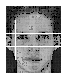
\includegraphics{pics/face.png}

\cvfunc{InitMixSegm}

Segments all observations within every internal state of HMM by state mixture components

\cvexp{
void cvInitMixSegm( \par CvImgObsInfo** obsInfoArray, \par int numImg, \par CvEHMM* hmm );

}{CPP}{PYTHON}

\begin{description}
\cvarg{obsInfoArray}{Array of pointers to the observation structures.}
\cvarg{numImg}{Length of above array.}
\cvarg{hmm}{HMM.}
\end{description}

The function \texttt{cvInitMixSegm} takes a group of observations from several training images already segmented by states and splits a set of observation vectors within every internal HMM state into as many clusters as the number of mixture components in the state.

\cvfunc{EstimateHMMStateParams}

Estimates all parameters of every HMM state

\cvexp{
void cvEstimateHMMStateParams( \par CvImgObsInfo** obsInfoArray, \par int numImg, \par CvEHMM* hmm );

}{CPP}{PYTHON}

\begin{description}
\cvarg{obsInfoArray}{Array of pointers to the observation structures.}
\cvarg{numImg}{Length of the array.}
\cvarg{hmm}{HMM.}
\end{description}

The function \texttt{cvEstimateHMMStateParams} computes all inner parameters of every HMM state, including Gaussian means, variances, etc.

\cvfunc{EstimateTransProb}

Computes transition probability matrices for embedded HMM

\cvexp{
void cvEstimateTransProb( \par CvImgObsInfo** obsInfoArray, \par int numImg, \par CvEHMM* hmm );

}{CPP}{PYTHON}

\begin{description}
\cvarg{obsInfoArray}{Array of pointers to the observation structures.}
\cvarg{numImg}{Length of the above array.}
\cvarg{hmm}{HMM.}
\end{description}

The function \texttt{cvEstimateTransProb} uses current segmentation of image observations to compute transition probability matrices for all embedded and external HMMs.

\cvfunc{EstimateObsProb}

Computes probability of every observation of several images

\cvexp{
void cvEstimateObsProb( CvImgObsInfo* obsInfo, CvEHMM* hmm );

}{CPP}{PYTHON}

\begin{description}
\cvarg{obsInfo}{Observation structure.}
\cvarg{hmm}{HMM structure.}
\end{description}

The function \texttt{cvEstimateObsProb} computes Gaussian probabilities of each observation to occur in each of the internal HMM states.

\cvfunc{EViterbi}

Executes Viterbi algorithm for embedded HMM

\cvexp{
float cvEViterbi( CvImgObsInfo* obsInfo, CvEHMM* hmm );

}{CPP}{PYTHON}

\begin{description}
\cvarg{obsInfo}{Observation structure.
}\cvarg{hmm}{HMM structure.}
\end{description}

The function \texttt{cvEViterbi} executes Viterbi algorithm for embedded HMM. Viterbi algorithm evaluates the likelihood of the best match between the given image observations and the given HMM and performs segmentation of image observations by HMM states. The segmentation is done on the basis of the match found.

\cvfunc{MixSegmL2}

Segments observations from all training images by mixture components of newly assigned states

\cvexp{
void cvMixSegmL2( \par CvImgObsInfo** obsInfoArray, \par int numImg, \par CvEHMM* hmm );

}{CPP}{PYTHON}

\begin{description}
\cvarg{obsInfoArray}{Array of pointers to the observation structures.}
\cvarg{numImg}{Length of the array.}
\cvarg{hmm}{HMM.}
\end{description}

The function \texttt{cvMixSegmL2} segments observations from all training images by mixture components of newly Viterbi algorithm-assigned states. The function uses Euclidean distance to group vectors around the existing mixtures centers.

